% Options for packages loaded elsewhere
\PassOptionsToPackage{unicode}{hyperref}
\PassOptionsToPackage{hyphens}{url}
\PassOptionsToPackage{dvipsnames,svgnames,x11names}{xcolor}
%
\documentclass[
  letterpaper,
  DIV=11,
  numbers=noendperiod]{scrartcl}

\usepackage{amsmath,amssymb}
\usepackage{iftex}
\ifPDFTeX
  \usepackage[T1]{fontenc}
  \usepackage[utf8]{inputenc}
  \usepackage{textcomp} % provide euro and other symbols
\else % if luatex or xetex
  \usepackage{unicode-math}
  \defaultfontfeatures{Scale=MatchLowercase}
  \defaultfontfeatures[\rmfamily]{Ligatures=TeX,Scale=1}
\fi
\usepackage{lmodern}
\ifPDFTeX\else  
    % xetex/luatex font selection
\fi
% Use upquote if available, for straight quotes in verbatim environments
\IfFileExists{upquote.sty}{\usepackage{upquote}}{}
\IfFileExists{microtype.sty}{% use microtype if available
  \usepackage[]{microtype}
  \UseMicrotypeSet[protrusion]{basicmath} % disable protrusion for tt fonts
}{}
\makeatletter
\@ifundefined{KOMAClassName}{% if non-KOMA class
  \IfFileExists{parskip.sty}{%
    \usepackage{parskip}
  }{% else
    \setlength{\parindent}{0pt}
    \setlength{\parskip}{6pt plus 2pt minus 1pt}}
}{% if KOMA class
  \KOMAoptions{parskip=half}}
\makeatother
\usepackage{xcolor}
\setlength{\emergencystretch}{3em} % prevent overfull lines
\setcounter{secnumdepth}{-\maxdimen} % remove section numbering
% Make \paragraph and \subparagraph free-standing
\makeatletter
\ifx\paragraph\undefined\else
  \let\oldparagraph\paragraph
  \renewcommand{\paragraph}{
    \@ifstar
      \xxxParagraphStar
      \xxxParagraphNoStar
  }
  \newcommand{\xxxParagraphStar}[1]{\oldparagraph*{#1}\mbox{}}
  \newcommand{\xxxParagraphNoStar}[1]{\oldparagraph{#1}\mbox{}}
\fi
\ifx\subparagraph\undefined\else
  \let\oldsubparagraph\subparagraph
  \renewcommand{\subparagraph}{
    \@ifstar
      \xxxSubParagraphStar
      \xxxSubParagraphNoStar
  }
  \newcommand{\xxxSubParagraphStar}[1]{\oldsubparagraph*{#1}\mbox{}}
  \newcommand{\xxxSubParagraphNoStar}[1]{\oldsubparagraph{#1}\mbox{}}
\fi
\makeatother

\usepackage{color}
\usepackage{fancyvrb}
\newcommand{\VerbBar}{|}
\newcommand{\VERB}{\Verb[commandchars=\\\{\}]}
\DefineVerbatimEnvironment{Highlighting}{Verbatim}{commandchars=\\\{\}}
% Add ',fontsize=\small' for more characters per line
\usepackage{framed}
\definecolor{shadecolor}{RGB}{241,243,245}
\newenvironment{Shaded}{\begin{snugshade}}{\end{snugshade}}
\newcommand{\AlertTok}[1]{\textcolor[rgb]{0.68,0.00,0.00}{#1}}
\newcommand{\AnnotationTok}[1]{\textcolor[rgb]{0.37,0.37,0.37}{#1}}
\newcommand{\AttributeTok}[1]{\textcolor[rgb]{0.40,0.45,0.13}{#1}}
\newcommand{\BaseNTok}[1]{\textcolor[rgb]{0.68,0.00,0.00}{#1}}
\newcommand{\BuiltInTok}[1]{\textcolor[rgb]{0.00,0.23,0.31}{#1}}
\newcommand{\CharTok}[1]{\textcolor[rgb]{0.13,0.47,0.30}{#1}}
\newcommand{\CommentTok}[1]{\textcolor[rgb]{0.37,0.37,0.37}{#1}}
\newcommand{\CommentVarTok}[1]{\textcolor[rgb]{0.37,0.37,0.37}{\textit{#1}}}
\newcommand{\ConstantTok}[1]{\textcolor[rgb]{0.56,0.35,0.01}{#1}}
\newcommand{\ControlFlowTok}[1]{\textcolor[rgb]{0.00,0.23,0.31}{\textbf{#1}}}
\newcommand{\DataTypeTok}[1]{\textcolor[rgb]{0.68,0.00,0.00}{#1}}
\newcommand{\DecValTok}[1]{\textcolor[rgb]{0.68,0.00,0.00}{#1}}
\newcommand{\DocumentationTok}[1]{\textcolor[rgb]{0.37,0.37,0.37}{\textit{#1}}}
\newcommand{\ErrorTok}[1]{\textcolor[rgb]{0.68,0.00,0.00}{#1}}
\newcommand{\ExtensionTok}[1]{\textcolor[rgb]{0.00,0.23,0.31}{#1}}
\newcommand{\FloatTok}[1]{\textcolor[rgb]{0.68,0.00,0.00}{#1}}
\newcommand{\FunctionTok}[1]{\textcolor[rgb]{0.28,0.35,0.67}{#1}}
\newcommand{\ImportTok}[1]{\textcolor[rgb]{0.00,0.46,0.62}{#1}}
\newcommand{\InformationTok}[1]{\textcolor[rgb]{0.37,0.37,0.37}{#1}}
\newcommand{\KeywordTok}[1]{\textcolor[rgb]{0.00,0.23,0.31}{\textbf{#1}}}
\newcommand{\NormalTok}[1]{\textcolor[rgb]{0.00,0.23,0.31}{#1}}
\newcommand{\OperatorTok}[1]{\textcolor[rgb]{0.37,0.37,0.37}{#1}}
\newcommand{\OtherTok}[1]{\textcolor[rgb]{0.00,0.23,0.31}{#1}}
\newcommand{\PreprocessorTok}[1]{\textcolor[rgb]{0.68,0.00,0.00}{#1}}
\newcommand{\RegionMarkerTok}[1]{\textcolor[rgb]{0.00,0.23,0.31}{#1}}
\newcommand{\SpecialCharTok}[1]{\textcolor[rgb]{0.37,0.37,0.37}{#1}}
\newcommand{\SpecialStringTok}[1]{\textcolor[rgb]{0.13,0.47,0.30}{#1}}
\newcommand{\StringTok}[1]{\textcolor[rgb]{0.13,0.47,0.30}{#1}}
\newcommand{\VariableTok}[1]{\textcolor[rgb]{0.07,0.07,0.07}{#1}}
\newcommand{\VerbatimStringTok}[1]{\textcolor[rgb]{0.13,0.47,0.30}{#1}}
\newcommand{\WarningTok}[1]{\textcolor[rgb]{0.37,0.37,0.37}{\textit{#1}}}

\providecommand{\tightlist}{%
  \setlength{\itemsep}{0pt}\setlength{\parskip}{0pt}}\usepackage{longtable,booktabs,array}
\usepackage{calc} % for calculating minipage widths
% Correct order of tables after \paragraph or \subparagraph
\usepackage{etoolbox}
\makeatletter
\patchcmd\longtable{\par}{\if@noskipsec\mbox{}\fi\par}{}{}
\makeatother
% Allow footnotes in longtable head/foot
\IfFileExists{footnotehyper.sty}{\usepackage{footnotehyper}}{\usepackage{footnote}}
\makesavenoteenv{longtable}
\usepackage{graphicx}
\makeatletter
\def\maxwidth{\ifdim\Gin@nat@width>\linewidth\linewidth\else\Gin@nat@width\fi}
\def\maxheight{\ifdim\Gin@nat@height>\textheight\textheight\else\Gin@nat@height\fi}
\makeatother
% Scale images if necessary, so that they will not overflow the page
% margins by default, and it is still possible to overwrite the defaults
% using explicit options in \includegraphics[width, height, ...]{}
\setkeys{Gin}{width=\maxwidth,height=\maxheight,keepaspectratio}
% Set default figure placement to htbp
\makeatletter
\def\fps@figure{htbp}
\makeatother

\KOMAoption{captions}{tableheading}
\makeatletter
\@ifpackageloaded{caption}{}{\usepackage{caption}}
\AtBeginDocument{%
\ifdefined\contentsname
  \renewcommand*\contentsname{Table of contents}
\else
  \newcommand\contentsname{Table of contents}
\fi
\ifdefined\listfigurename
  \renewcommand*\listfigurename{List of Figures}
\else
  \newcommand\listfigurename{List of Figures}
\fi
\ifdefined\listtablename
  \renewcommand*\listtablename{List of Tables}
\else
  \newcommand\listtablename{List of Tables}
\fi
\ifdefined\figurename
  \renewcommand*\figurename{Figure}
\else
  \newcommand\figurename{Figure}
\fi
\ifdefined\tablename
  \renewcommand*\tablename{Table}
\else
  \newcommand\tablename{Table}
\fi
}
\@ifpackageloaded{float}{}{\usepackage{float}}
\floatstyle{ruled}
\@ifundefined{c@chapter}{\newfloat{codelisting}{h}{lop}}{\newfloat{codelisting}{h}{lop}[chapter]}
\floatname{codelisting}{Listing}
\newcommand*\listoflistings{\listof{codelisting}{List of Listings}}
\makeatother
\makeatletter
\makeatother
\makeatletter
\@ifpackageloaded{caption}{}{\usepackage{caption}}
\@ifpackageloaded{subcaption}{}{\usepackage{subcaption}}
\makeatother

\ifLuaTeX
  \usepackage{selnolig}  % disable illegal ligatures
\fi
\usepackage{bookmark}

\IfFileExists{xurl.sty}{\usepackage{xurl}}{} % add URL line breaks if available
\urlstyle{same} % disable monospaced font for URLs
\hypersetup{
  pdftitle={Homework 1 \textbar{} STAT 330},
  pdfauthor={Marshall Nielsen},
  colorlinks=true,
  linkcolor={blue},
  filecolor={Maroon},
  citecolor={Blue},
  urlcolor={Blue},
  pdfcreator={LaTeX via pandoc}}


\title{Homework 1 \textbar{} STAT 330}
\usepackage{etoolbox}
\makeatletter
\providecommand{\subtitle}[1]{% add subtitle to \maketitle
  \apptocmd{\@title}{\par {\large #1 \par}}{}{}
}
\makeatother
\subtitle{Simple Linear Regression}
\author{Marshall Nielsen}
\date{}

\begin{document}
\maketitle


\subsection{Data and Description}\label{data-and-description}

Energy can be produced from wind using windmills. Choosing a site for a
wind farm (i.e.~the location of the windmills), however, can be a
multi-million dollar gamble. If wind is inadequate at the site, then the
energy produced over the lifetime of the wind farm can be much less than
the cost of building the operation. Hence, accurate prediction of wind
speed at a candidate site can be an important component in the decision
to build or not to build. Because the energy produced is proportional to
the square of the wind speed, even small errors in wind speed prediction
can lead to significant impacts.

A potential approach for predicting wind speed at a candidate site is to
use wind speed data from a nearby reference site. A reference site is a
nearby location where the wind speed is already being monitored and
should, theoretically, be similar to the candidate site. If the
reference sites turn out to be good predictors of the candidate sites,
leveraging the information from the reference site would allow windmill
companies to estimate the wind speed at the candidate sites without
going through a costly and lengthy data collection period.

The Windmill data set contains measurements of wind speed (in meters per
second m/s) at \textbf{candidate sites (CSpd) (column 1)} and at
corresponding \textbf{reference sites (RSpd) (column 2)} for 1,116
sites. Download the Windmill.txt file from Canvas (which can be found in
Files -\textgreater{} Data Sets), and put it in the same folder as this
quarto file.

\paragraph{\texorpdfstring{0. Replace the text ``\textless{} PUT YOUR
NAME HERE \textgreater{}'' (above next to ``author:'') with your full
name.}{0. Replace the text ``\textless{} PUT YOUR NAME HERE \textgreater'' (above next to ``author:'') with your full name.}}\label{replace-the-text-put-your-name-here-above-next-to-author-with-your-full-name.}

\paragraph{1. Briefly explain why simple linear regression could be a
useful tool for this
problem.}\label{briefly-explain-why-simple-linear-regression-could-be-a-useful-tool-for-this-problem.}

Simple linear regression would be a useful tool for this problem because
we want to investigate the nature of the relationship between the wind
speeds at candidate sites and their corresponding reference sites. This
means that we have one variable and one response, making simple linear
regression appropriate.

\paragraph{2. Read in the data set into an object named ``wind''.
Display the first 6 rows of the
data.}\label{read-in-the-data-set-into-an-object-named-wind.-display-the-first-6-rows-of-the-data.}

\begin{Shaded}
\begin{Highlighting}[]
\NormalTok{windmill\_data }\OtherTok{\textless{}{-}} \FunctionTok{read.table}\NormalTok{(}\StringTok{"Windmill.txt"}\NormalTok{, }\AttributeTok{header =} \ConstantTok{TRUE}\NormalTok{)}
\FunctionTok{head}\NormalTok{(windmill\_data)}
\end{Highlighting}
\end{Shaded}

\begin{verbatim}
  CSpd   RSpd
1  6.9 5.9666
2  7.1 7.2176
3  7.8 7.9405
4  6.9 6.0174
5  5.5 6.1646
6  3.1 1.7687
\end{verbatim}

\paragraph{3. What is the response/outcome variable in this situation?
(Think about which variable makes the most sense to be the
response.)}\label{what-is-the-responseoutcome-variable-in-this-situation-think-about-which-variable-makes-the-most-sense-to-be-the-response.}

The wind speed at the candidate sites, or the CSpd column.

\paragraph{4. What is the explanatory variable in this
situation?}\label{what-is-the-explanatory-variable-in-this-situation}

The wind speed at the reference sites, or the RSpd column.

\paragraph{5. Create a scatterplot of the data with variables on the
appropriate axes. Add descriptive axis labels with appropriate units.
Display the
plot.}\label{create-a-scatterplot-of-the-data-with-variables-on-the-appropriate-axes.-add-descriptive-axis-labels-with-appropriate-units.-display-the-plot.}

\begin{Shaded}
\begin{Highlighting}[]
\CommentTok{\#Got some help here for creating a scatter plot using ggplot from chatgpt}

\FunctionTok{library}\NormalTok{(ggplot2)}

\CommentTok{\# Create scatter plot with labels}
\NormalTok{plot }\OtherTok{\textless{}{-}} \FunctionTok{ggplot}\NormalTok{(windmill\_data, }\FunctionTok{aes}\NormalTok{(}\AttributeTok{x =}\NormalTok{ RSpd, }\AttributeTok{y =}\NormalTok{ CSpd)) }\SpecialCharTok{+}
  \FunctionTok{geom\_point}\NormalTok{(}\AttributeTok{color =} \StringTok{"blue"}\NormalTok{, }\AttributeTok{size =} \DecValTok{1}\NormalTok{) }\SpecialCharTok{+}
  \FunctionTok{labs}\NormalTok{(}\AttributeTok{title =} \StringTok{"The Relationship Between Wind Speeds at Reference Sites and Candidate Sites"}\NormalTok{,}
       \AttributeTok{x =} \StringTok{"Reference Site Wind Speed (m/s)"}\NormalTok{,}
       \AttributeTok{y =} \StringTok{"Candidate Site Wind Speed (m/s)"}\NormalTok{) }\SpecialCharTok{+}
  \FunctionTok{theme\_minimal}\NormalTok{()}

\CommentTok{\# Print the plot}
\FunctionTok{print}\NormalTok{(plot)}
\end{Highlighting}
\end{Shaded}

\begin{center}
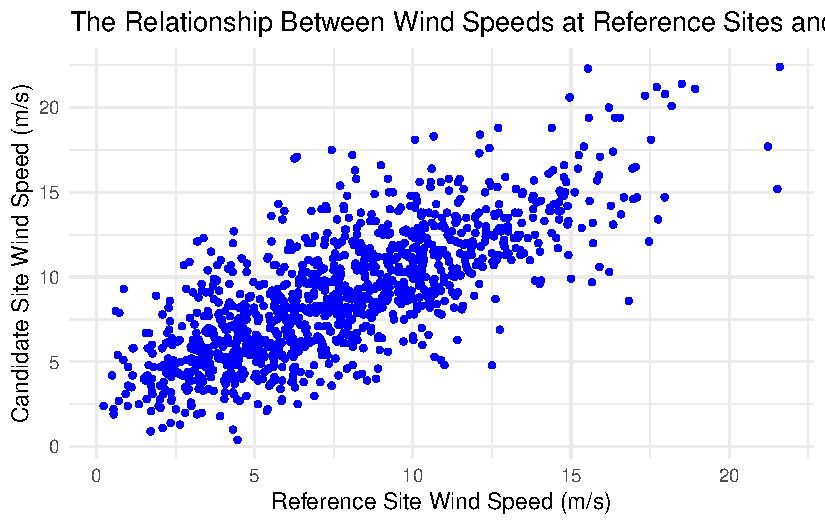
\includegraphics{HW_1_files/figure-pdf/unnamed-chunk-2-1.pdf}
\end{center}

\paragraph{6. Briefly describe the relationship between RSpd and CSpd in
terms of its linearity, direction, and
strength.}\label{briefly-describe-the-relationship-between-rspd-and-cspd-in-terms-of-its-linearity-direction-and-strength.}

It seems to be a clear linear relationship in a positive direction, but
it isn't as strong as it could be.

\paragraph{7. Calculate the correlation coefficient for the two
variables (you may use a built-in R function). Display the
result.}\label{calculate-the-correlation-coefficient-for-the-two-variables-you-may-use-a-built-in-r-function.-display-the-result.}

\begin{Shaded}
\begin{Highlighting}[]
\FunctionTok{print}\NormalTok{(}\FunctionTok{cor}\NormalTok{(windmill\_data}\SpecialCharTok{$}\NormalTok{CSpd, windmill\_data}\SpecialCharTok{$}\NormalTok{RSpd))}
\end{Highlighting}
\end{Shaded}

\begin{verbatim}
[1] 0.7555948
\end{verbatim}

\paragraph{8. What does the calculated correlation coefficient tell you
about the direction and strength of the linear association between these
two
variables?}\label{what-does-the-calculated-correlation-coefficient-tell-you-about-the-direction-and-strength-of-the-linear-association-between-these-two-variables}

It tells me that it is a strong positive linear correlation.

\paragraph{\texorpdfstring{9. The equation below shows the generic
\textbf{theoretical} simple linear regression model. Update the equation
to use variable names that are meaningful in context of this dataset
(i.e., rename ``x'' and
``y'').}{9. The equation below shows the generic theoretical simple linear regression model. Update the equation to use variable names that are meaningful in context of this dataset (i.e., rename ``x'' and ``y'').}}\label{the-equation-below-shows-the-generic-theoretical-simple-linear-regression-model.-update-the-equation-to-use-variable-names-that-are-meaningful-in-context-of-this-dataset-i.e.-rename-x-and-y.}

\[\begin{align}
    CSpd &= \beta_0 + \beta_1 \times RSpd + \epsilon_i \\ 
    \epsilon_i &\stackrel{iid}{\sim} N(0, \sigma^2) 
    \end{align} \]

\paragraph{\texorpdfstring{10. Add the OLS regression line to the
scatterplot you created in 5. Display the result. (If you use
\texttt{ggplot} with \texttt{geom\_smooth}, You can remove the standard
error line with the option
\texttt{se\ =\ FALSE}).}{10. Add the OLS regression line to the scatterplot you created in 5. Display the result. (If you use ggplot with geom\_smooth, You can remove the standard error line with the option se = FALSE).}}\label{add-the-ols-regression-line-to-the-scatterplot-you-created-in-5.-display-the-result.-if-you-use-ggplot-with-geom_smooth-you-can-remove-the-standard-error-line-with-the-option-se-false.}

\begin{Shaded}
\begin{Highlighting}[]
\NormalTok{plot }\OtherTok{\textless{}{-}} \FunctionTok{ggplot}\NormalTok{(windmill\_data, }\FunctionTok{aes}\NormalTok{(}\AttributeTok{x =}\NormalTok{ RSpd, }\AttributeTok{y =}\NormalTok{ CSpd)) }\SpecialCharTok{+}
  \FunctionTok{geom\_point}\NormalTok{(}\AttributeTok{color =} \StringTok{"blue"}\NormalTok{, }\AttributeTok{size =} \DecValTok{1}\NormalTok{) }\SpecialCharTok{+}
  \FunctionTok{labs}\NormalTok{(}\AttributeTok{title =} \StringTok{"The Relationship Between Wind Speeds at Reference Sites and Candidate Sites"}\NormalTok{,}
       \AttributeTok{x =} \StringTok{"Reference Site Wind Speed (m/s)"}\NormalTok{,}
       \AttributeTok{y =} \StringTok{"Candidate Site Wind Speed (m/s)"}\NormalTok{) }\SpecialCharTok{+}
  \FunctionTok{geom\_smooth}\NormalTok{(}\AttributeTok{method =} \StringTok{"lm"}\NormalTok{, }\AttributeTok{formula =}\NormalTok{ y }\SpecialCharTok{\textasciitilde{}}\NormalTok{ x, }\AttributeTok{se =} \ConstantTok{FALSE}\NormalTok{) }\SpecialCharTok{+}
  \FunctionTok{theme\_minimal}\NormalTok{()}

\FunctionTok{print}\NormalTok{(plot)}
\end{Highlighting}
\end{Shaded}

\begin{center}
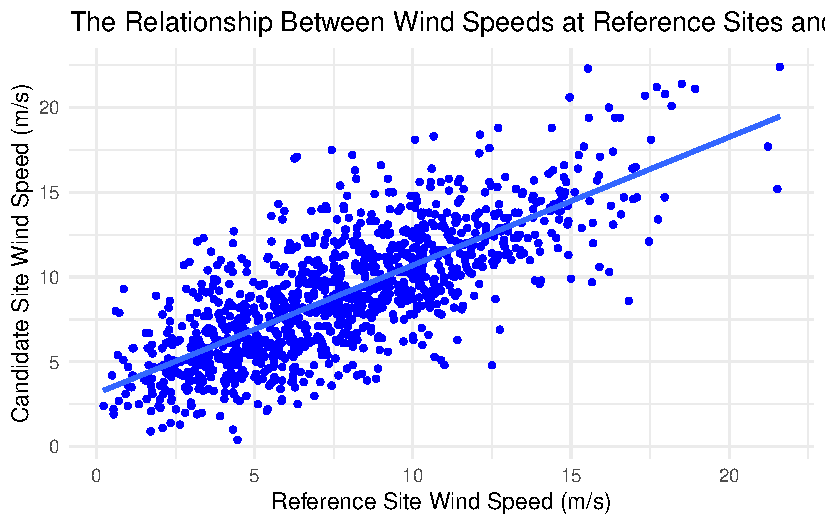
\includegraphics{HW_1_files/figure-pdf/unnamed-chunk-4-1.pdf}
\end{center}

\paragraph{\texorpdfstring{11. (a) Apply linear regression to the data.
(b) Display a summary of the results from the \texttt{lm} function. (c)
Plot the model residuals against fitted values in a well-labeled
scatterplot.}{11. (a) Apply linear regression to the data. (b) Display a summary of the results from the lm function. (c) Plot the model residuals against fitted values in a well-labeled scatterplot.}}\label{a-apply-linear-regression-to-the-data.-b-display-a-summary-of-the-results-from-the-lm-function.-c-plot-the-model-residuals-against-fitted-values-in-a-well-labeled-scatterplot.}

\begin{Shaded}
\begin{Highlighting}[]
\NormalTok{linear\_regression }\OtherTok{\textless{}{-}} \FunctionTok{lm}\NormalTok{(CSpd }\SpecialCharTok{\textasciitilde{}}\NormalTok{ RSpd, }\AttributeTok{data =}\NormalTok{ windmill\_data)}
\FunctionTok{summary}\NormalTok{(linear\_regression)}
\end{Highlighting}
\end{Shaded}

\begin{verbatim}

Call:
lm(formula = CSpd ~ RSpd, data = windmill_data)

Residuals:
    Min      1Q  Median      3Q     Max 
-7.7877 -1.5864 -0.1994  1.4403  9.1738 

Coefficients:
            Estimate Std. Error t value Pr(>|t|)    
(Intercept)  3.14123    0.16958   18.52   <2e-16 ***
RSpd         0.75573    0.01963   38.50   <2e-16 ***
---
Signif. codes:  0 '***' 0.001 '**' 0.01 '*' 0.05 '.' 0.1 ' ' 1

Residual standard error: 2.466 on 1114 degrees of freedom
Multiple R-squared:  0.5709,    Adjusted R-squared:  0.5705 
F-statistic:  1482 on 1 and 1114 DF,  p-value: < 2.2e-16
\end{verbatim}

\begin{Shaded}
\begin{Highlighting}[]
\NormalTok{fitted\_values }\OtherTok{\textless{}{-}} \FunctionTok{fitted}\NormalTok{(linear\_regression)}
\NormalTok{residuals }\OtherTok{\textless{}{-}} \FunctionTok{residuals}\NormalTok{(linear\_regression)}

\NormalTok{plot }\OtherTok{\textless{}{-}} \FunctionTok{ggplot}\NormalTok{(}\AttributeTok{data =} \FunctionTok{data.frame}\NormalTok{(fitted\_values, residuals), }\FunctionTok{aes}\NormalTok{(}\AttributeTok{x =}\NormalTok{ fitted\_values, }\AttributeTok{y =}\NormalTok{ residuals)) }\SpecialCharTok{+}
  \FunctionTok{geom\_point}\NormalTok{(}\AttributeTok{color =} \StringTok{"blue"}\NormalTok{, }\AttributeTok{size =} \DecValTok{1}\NormalTok{) }\SpecialCharTok{+}
  \FunctionTok{labs}\NormalTok{(}\AttributeTok{title =} \StringTok{"Plotting the Residuals Against the Corresponding Fitted Values"}\NormalTok{,}
       \AttributeTok{x =} \StringTok{"Fitted Values"}\NormalTok{,}
       \AttributeTok{y =} \StringTok{"Residuals"}\NormalTok{) }\SpecialCharTok{+}
  \FunctionTok{geom\_smooth}\NormalTok{(}\AttributeTok{method =} \StringTok{"lm"}\NormalTok{, }\AttributeTok{formula =}\NormalTok{ y }\SpecialCharTok{\textasciitilde{}}\NormalTok{ x, }\AttributeTok{se =} \ConstantTok{FALSE}\NormalTok{) }\SpecialCharTok{+}
  \FunctionTok{theme\_minimal}\NormalTok{()}

\FunctionTok{print}\NormalTok{(plot)}
\end{Highlighting}
\end{Shaded}

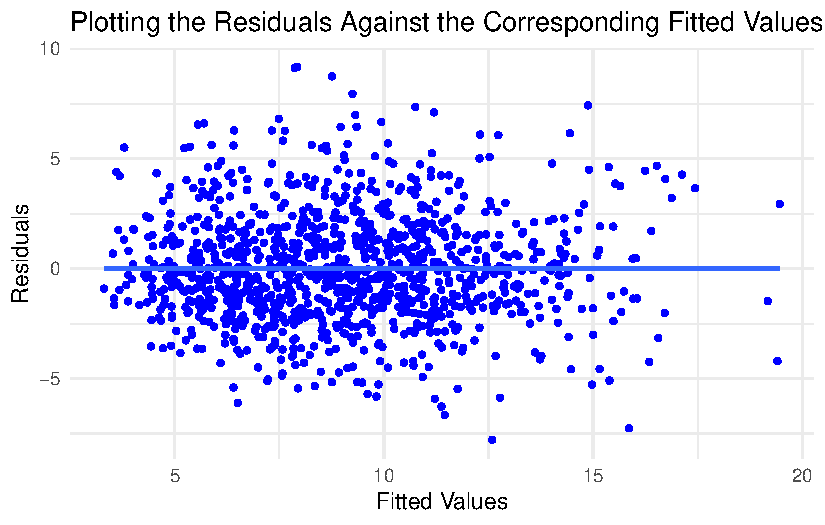
\includegraphics{HW_1_files/figure-pdf/unnamed-chunk-5-1.pdf}

\paragraph{\texorpdfstring{12. Update the fitted simple linear
regression model shown below with the coefficients you obtained from
your linear model (i.e., update the \(\hat{\beta}\)s with specific
numeric values). Round to two decimal
places.}{12. Update the fitted simple linear regression model shown below with the coefficients you obtained from your linear model (i.e., update the \textbackslash hat\{\textbackslash beta\}s with specific numeric values). Round to two decimal places.}}\label{update-the-fitted-simple-linear-regression-model-shown-below-with-the-coefficients-you-obtained-from-your-linear-model-i.e.-update-the-hatbetas-with-specific-numeric-values.-round-to-two-decimal-places.}

\[\widehat{\text{Cand Speed}}_i = 3.14 + 0.76 \times \text{Ref Speed}_i.\]

\paragraph{13. Interpret the coefficient for the
slope.}\label{interpret-the-coefficient-for-the-slope.}

This means that for every 1 m/s increase in the wind speed at the
reference site, there tends to be a 0.76 m/s increase in wind speed at
the candidate site.

\paragraph{14. Interpret the coefficient for the
intercept.}\label{interpret-the-coefficient-for-the-intercept.}

This means that if there were no wind at the reference site, the wind at
the candidate site would tend to be about 3.14 m/s.

\paragraph{15. What is the estimated average wind speed at the candidate
site (CSpd) when the wind speed at the reference site (RSpd) is 12 m/s?
Show your code, and display the
result.}\label{what-is-the-estimated-average-wind-speed-at-the-candidate-site-cspd-when-the-wind-speed-at-the-reference-site-rspd-is-12-ms-show-your-code-and-display-the-result.}

\begin{Shaded}
\begin{Highlighting}[]
\NormalTok{RSpd }\OtherTok{\textless{}{-}} \FunctionTok{c}\NormalTok{(}\DecValTok{12}\NormalTok{)}
\NormalTok{prediction }\OtherTok{\textless{}{-}} \FunctionTok{predict}\NormalTok{(linear\_regression, }\AttributeTok{newdata =} \FunctionTok{data.frame}\NormalTok{(RSpd))}
\FunctionTok{print}\NormalTok{(prediction)}
\end{Highlighting}
\end{Shaded}

\begin{verbatim}
       1 
12.21003 
\end{verbatim}

\paragraph{16. Briefly explain why it would be inadvisable to answer
this question using your model: What is the estimated average wind speed
at the candidate site (CSpd) when the wind speed at the reference site
(RSpd) is 25
m/s?}\label{briefly-explain-why-it-would-be-inadvisable-to-answer-this-question-using-your-model-what-is-the-estimated-average-wind-speed-at-the-candidate-site-cspd-when-the-wind-speed-at-the-reference-site-rspd-is-25-ms}

It would be inadvisable because while we could make a prediction, we
don't have any points that are close to that wind speed that were used
to make the model, and so there could be a different relationship
between variable and response when the wind is blowing that hard -- we
just don't know.

\paragraph{\texorpdfstring{17. Calculate the (unbiased) estimate of
\(\sigma^2\). Show your code, and display the
result.}{17. Calculate the (unbiased) estimate of \textbackslash sigma\^{}2. Show your code, and display the result.}}\label{calculate-the-unbiased-estimate-of-sigma2.-show-your-code-and-display-the-result.}

\begin{Shaded}
\begin{Highlighting}[]
\NormalTok{sigma\_squared }\OtherTok{\textless{}{-}} \FunctionTok{summary}\NormalTok{(linear\_regression)}\SpecialCharTok{$}\NormalTok{sigma}\SpecialCharTok{\^{}}\DecValTok{2}
\FunctionTok{print}\NormalTok{(sigma\_squared)}
\end{Highlighting}
\end{Shaded}

\begin{verbatim}
[1] 6.082312
\end{verbatim}

\paragraph{18. Create the design matrix for your model and store it in a
variable. Display the first few rows of the design
matrix.}\label{create-the-design-matrix-for-your-model-and-store-it-in-a-variable.-display-the-first-few-rows-of-the-design-matrix.}

\begin{Shaded}
\begin{Highlighting}[]
\NormalTok{design\_matrix }\OtherTok{\textless{}{-}} \FunctionTok{model.matrix}\NormalTok{(linear\_regression)}
\FunctionTok{head}\NormalTok{(design\_matrix)}
\end{Highlighting}
\end{Shaded}

\begin{verbatim}
  (Intercept)   RSpd
1           1 5.9666
2           1 7.2176
3           1 7.9405
4           1 6.0174
5           1 6.1646
6           1 1.7687
\end{verbatim}

\paragraph{19. Obtain the parameter estimates for this same model using
matrix multiplication. You should use the following in your
computations: t() {[}transpose{]}, solve() {[}inverse{]}, and \%*\%
{[}matrix multiplicaton{]}. Display the
result.}\label{obtain-the-parameter-estimates-for-this-same-model-using-matrix-multiplication.-you-should-use-the-following-in-your-computations-t-transpose-solve-inverse-and-matrix-multiplicaton.-display-the-result.}

\begin{Shaded}
\begin{Highlighting}[]
\NormalTok{X }\OtherTok{\textless{}{-}}\NormalTok{ design\_matrix}
\NormalTok{y }\OtherTok{\textless{}{-}}\NormalTok{ windmill\_data}\SpecialCharTok{$}\NormalTok{CSpd}

\NormalTok{beta\_hat }\OtherTok{\textless{}{-}} \FunctionTok{solve}\NormalTok{((}\FunctionTok{t}\NormalTok{(X) }\SpecialCharTok{\%*\%}\NormalTok{ X)) }\SpecialCharTok{\%*\%}\NormalTok{ (}\FunctionTok{t}\NormalTok{(X) }\SpecialCharTok{\%*\%}\NormalTok{ y)}
\FunctionTok{print}\NormalTok{(beta\_hat)}
\end{Highlighting}
\end{Shaded}

\begin{verbatim}
                 [,1]
(Intercept) 3.1412324
RSpd        0.7557333
\end{verbatim}

\paragraph{20. Briefly summarize what you learned, personally, from this
analysis about statistics, the model fitting process, R,
etc.}\label{briefly-summarize-what-you-learned-personally-from-this-analysis-about-statistics-the-model-fitting-process-r-etc.}

I do a lot of model fitting in Python for my job, but it was good to
learn how to do it in R, and that it isn't so different. It was helpful
to see the different ways that we can leverage the functions and
attributes to arrive at our estimations for the Beta values, which I'm
thinking might be useful in different situations where we're using
regressions at different points in the modeling process.

\paragraph{\texorpdfstring{21. Briefly summarize what you learned about
the scientific question from this analysis \emph{to a non-statistician}.
Write a few sentences about (1) the purpose of this data set and
analysis and (2) what you learned about this data set from your
analysis. Write your response as if you were addressing a business
manager (avoid using statistics jargon) and just provide the main
take-aways.}{21. Briefly summarize what you learned about the scientific question from this analysis to a non-statistician. Write a few sentences about (1) the purpose of this data set and analysis and (2) what you learned about this data set from your analysis. Write your response as if you were addressing a business manager (avoid using statistics jargon) and just provide the main take-aways.}}\label{briefly-summarize-what-you-learned-about-the-scientific-question-from-this-analysis-to-a-non-statistician.-write-a-few-sentences-about-1-the-purpose-of-this-data-set-and-analysis-and-2-what-you-learned-about-this-data-set-from-your-analysis.-write-your-response-as-if-you-were-addressing-a-business-manager-avoid-using-statistics-jargon-and-just-provide-the-main-take-aways.}

For this study, we chose to analyze data on the relationship between the
wind speed at a candidate site for a wind farm and the wind speed at
reference sites nearby to explore the strength of the relationship
between the two. We found that there was a strong positive relationship
between the two wind speeds, and that for every meter per second faster
that the wind was blowing at a reference site, the wind would blow about
0.75 meters per second faster at the candidate site.




\end{document}
